\chapter{Monte Carlo Tree Search}
\label{ch_mcts}

Monte Carlo methods\footnote{Not to be confused with Monte Carlo
algorithms which are precisely defined as the algorithms solving the
decision problems in classes BPP and RP.} are using random sampling to
estimate a correct solution to a problem. The first practical use of Monte
Carlo methods was by Stanislaw Ulam and John von Neumann during their
work on the Manhattan project, but the technique has since spread into
many areas of science due to its general applicability.

One of the celebrated Monte Carlo methods
is the simulated annealing algorithm (so called due to its
origin in statistical physics) which is an improved version of
Metropolis algorithm (invented by a Manhattan project scientist
Nicholas C. Metropolis and others).

This method found its way into game
theory in 1993 when it was applied to the board game Go
\parencite{MonteCarloGo}. The approach was later further improved
\parencite{MonteCarloGoDevel}, but the real breakthrough came in 2006
when Coulom \parencite{Coulom} and Kocsis, Szepesvári \parencite{Kocsis}
independently explored the idea of maintaining a tree which would guide the
search for strategies -- thus discovering Monte Carlo Tree Search.
This was eventually used in the AlphaGo program
\parencite{alphago}, the first
computer program to beat professional human players.

Monte Carlo Tree Search (MCTS) is, in short, a
heuristic search algorithm for finding good strategies in complex
decision processes by combining standard approaches of artificial
intelligence and computational statistics: tree search and sampling.

In this chapter, the general MCTS scheme is defined, and a concrete instance
called UCT is shown together with its application to maximizing rewards
in MDPs and games. The chapter is based mostly on a thorough MCTS survey
paper \parencite{mcts_survey}.

Since the research into MCTS focuses mainly on using MCTS for reward
maximization, we demonstrate the algorithms on the reward maximization
problem too in this chapter unlike the rest of the thesis.

\section{General MCTS Scheme}

MCTS iteratively builds a tree which approximates possible rewards
attainable by strategies in the decision process. In each iteration, the
tree guides the search to balance between exploitation of known good
strategies and exploration of new strategies. When the search leaves the
tree, it adds one layer of new nodes, proceeds at random from one of the
new nodes, and upon terminating it updates the ancestors of the node
with the result.  The stages are usually called {\em selection}, {\em
expansion}, {\em simulation}, {\em backpropagation}.  The algorithm is
summarized in \autoref{mcts}.


\begin{algorithm}
\caption{General Monte Carlo Tree Search method}
\label{mcts}
\begin{algorithmic}
\Function{MCTS}{$s_0$}
    \State Let $v_0$ be the root of the MCTS tree, with $v_0.state = s_0$.
    \While{within computational budget}
        \State $v_l \gets \Call{TreePolicy}{v_0}$
        \State $r \gets \Call{Rollout}{v_l}$
        \State $\Call{Backup}{v_l, r}$
    \EndWhile
    \State \Return Action from $v_0$ to the best node (by some
    given metric).
\EndFunction
\end{algorithmic}
\end{algorithm}

Node $v_l$ is a leaf of the tree selected by the tree policy.
The leaf may be expanded -- the corresponding state's successors in the
MDP are then added as leafs.
A simulation (rollout) then starts from a new leaf.
$r$ is the reward gained by this rollout.

After the algorithm is interrupted and asked for a result or it runs out
of time, there are various ways how to
choose an action in the end, for example, the most visited child might
be chosen, or the child with the highest reward.


\pagebreak


\section{Upper Confidence Bound for Trees}

The most common implementation of the general scheme is {\em Upper
Confidence Bound for Trees} (UCT) which utilizes formula \ref{UCB} to
select nodes in the tree traversal.
In this formula $\overline{X}_i$ represents the expected outcome
from node $i$, $n$ is the number of visits to all nodes, $n_i$ is the
number of visits to node $i$. $C$ is an arbitrary constant.

\begin{equation}
\label{UCB}
UCT_i = \overline{X}_i + C \sqrt{ \frac{2 \ln n}{n_i} }
\end{equation}

The tree is traversed greedily, in every step a node with maximal UCT
value is chosen. By convention, unvisited nodes have their UCT value
equal to $\infty$.  Importantly, when a node $j$ is visited, its
sibling's $i$ UCT value is increased as $n$ increased but $n_i$ did not
-- this contributes to balance between exploitation of known good
strategies and exploration of new.  Constant $C$ instructs the algorithm
how much weight to give to exploration. See \parencite{improved_mc} for
insights into choice of $C$ in some specific situations.

\autoref{alg:uct} is an implementation of the general scheme of \autoref{mcts}.
As a minor simplification, the algorithm expects an MDP with rewards
$(S,s_0,A,E,R)$ and a marked set of terminal states, such that a reward
is paid out only when a terminal state is reached.

Every tree node $v$ has information about its corresponding state
($v.state$), the action which lead to it ($v.action$), the number of
times it has been visited so far ($v.visits$), and the reward which has
been collected after traversing through it ($v.q$, the Q refers to
Q-learning). For a node $v$ value $v.q / v.visits$ thus represents an
estimate of the actually attainable reward.

\begin{algorithm}
    \caption{Upper Confidence Bound for Trees}
\label{alg:uct}
\begin{algorithmic}
\Function{UCT}{$s_0$}
    \State Let $v_0$ be the root of the MCTS tree, with $v_0.state = s_0$.
    \While{within computational budget}
        \State $v_l \gets \Call{TreePolicy}{v_0}$
        \State $r \gets \Call{Rollout}{v_l}$
        \State $\Call{Backup}{v_l, r}$
    \EndWhile
    \State \Return $\Call{BestChild}{v_0, 0}.action$
\EndFunction

\Function{TreePolicy}{v}
    \While{$v$ is not terminal}
        \If{$v$ is not fully expanded}
            \State $\Call{Expand}{v}$
        \Else
            \State $v \gets \Call{BestChild}{v, C}$
        \EndIf
    \EndWhile
\EndFunction

\Function{Expand}{v}
    \State choose an untried action $a$ from $A(v.state)$
    \State add a new child $v'$ to $v$,
        $v'.state = \Delta(v.state, a),
        v'.action = a$
\EndFunction

\Function{BestChild}{v, C}
    \State \Return
    $\argmax\limits_{v' \text{ a child of } v}
    \frac{v'.q}{v'.visits} +
    C \sqrt{\frac{2\ln v.visits}{v'.visits}}$
\EndFunction

\Function{Rollout}{s}
    \While{$s$ is not terminal}
        \State choose $a \in E(s)$ uniformly at random
        \State $s \gets \Delta(s,a)$
    \EndWhile
    \Return reward for reaching $s$
\EndFunction

\Function{Backup}{s, r}
    \While{$v$ is not null}
        \State $v.visits \gets v.visits + 1$
        \State $v.q \gets v.q + r$
        \State $v \gets$ parent of $v$
    \EndWhile
\EndFunction
\end{algorithmic}
\end{algorithm}

The tree is the algorithm's estimate of the actual reward attainable
from various parts of the MDP. In each tree node
it greedily chooses to confirm it can get a good reward or goes to explore
a little explored part of the MDP, the choice depends on the tree heuristic value.
A random rollout is performed, and the algorithm then adds a new node to
the tree which allows for a more precise estimate in the chosen part of
the tree.

%As UCT is the most common type of MCTS algorithm, the terms UCT and MCTS
%are often used interchangeably in literature.

\section{Solving Games}

In this section a brief introduction to game theory is given, starting
with definitions of games, strategies, and solutions to games. We
proceed by presenting the standard {\em minimax} algorithm, then showing
how MCTS can be used to solve games and how it compares with minimax.
Lastly, we briefly compare the application of MCTS to Go and Chess.
Observing where it performs well and where it does not provides insight
the algorithm and it is a useful starting point for understanding the results
of evaluation in \autoref{ch_evaluation}.

We present the following definition for a precise understanding of games.
A reader can notice similarities with MDPs, for
example, games have states, actions and enabled actions, as well as
rewards, moreover, perfect information corresponds to complete
information. On the other hand, the transition function is
deterministic in our definition.

\begin{definition}
    A {\em perfect-information extensive-form game}
    is a tuple $G = (N, S, s_0, F, A, E, \Delta, \rho, u)$,
    where
    \begin{itemize}
        \item $N \subseteq \mathbb{N}$ is a set of $n$ players,
            for $n \in \mathbb{N}$,
        \item $S$ is a set of states,
        \item $s_0 \in S$ is the initial state,
        \item $F \subseteq S$ is a set of terminal states,
        \item $A$ is the set of actions,
        \item $E : S \to \mathcal{P}^+(A)$ is a function which tells the player
            which non-empty set of actions can be played in a given state,
        \item $\Delta : (S \setminus F) \times A \to A$ is the
            transition function, defined such that game states cannot
            repeat\footnote{
                Technically there are no $s \in S, a \in E(s)$ such that
                $\Delta(s,a) = s_0$, and for any two $s,s' \in S$ there
                are no actions $a \in E(s), a' \in E(s')$ such that
                $\Delta(s,a) = \Delta(s',a')$.
            },
        \item $\rho : S \to N$ is a function assigning who is on turn in
            a given state, %and finally
        \item $u = (u_1,\ldots,u_{n})$ is the tuple of
            utility (payoff, reward) functions where each $u_i, i \in N$
            is a function $u_i : F \to \mathbb{R}$.
    \end{itemize}
\end{definition}

Game starts in state $s_0$ and players take turns until
a terminal state (in $F$) is reached. In a turn a player in state $s$
chooses action $a$ from $E(s)$ and the action leads to state
$\Delta(s,a)$.  If the state $\Delta(s,a)$ is terminal, then every
player $i$ receives the reward $u_i(\Delta(s,a))$ and the game ends.

\begin{example}
A common choice of the utility function is $+1, 0, -1$ for victory, draw
and loss, respectively. Below is a depiction of such a game
in the usual way -- using a tree.
There are two players,
the nodes represent game states, leafs are the final states.
The root of the tree is the initial state.
Actions are given implicitly by choice of the next node.
Functions $E$ and $\Delta$ are given by the drawn edges.
$\rho$ is given by the color of the nodes
and the payoff function is represented by a tuple in each leaf.

\begin{center}
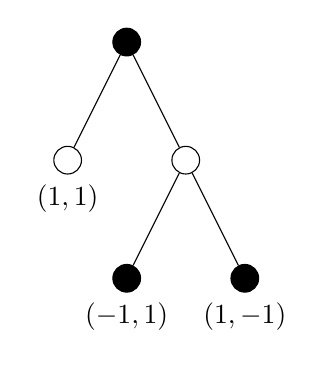
\begin{tikzpicture}
\tikzset{
solid node/.style={circle,draw,inner sep=1.5,minimum size=10pt,fill=black},
hollow node/.style={circle,draw,inner sep=1.5,minimum size=10pt}
}

\node(0)[solid node]{}
    child{node[hollow node,label=below:{$(1,1)$}]{}}
    child{node[hollow node]{}
        child{node[solid node,label=below:{$(-1,1)$}]{}}
        child{node[solid node,label=below:{$(1,-1)$}]{}}
    };
\end{tikzpicture}
\end{center}
\end{example}


\begin{definition}
    A {\em strategy} of player $i$ in a game $G$ is a function
    $\pi_i : S \to \distribution{A}$, such that for all $s \in S$ and $a
    \in A$ it holds that if $\pi_i(s)(a) > 0$ then $a \in E(s)$.

    A {\em strategy profile} is an $N$-tuple with a strategy for each player.
\end{definition}

We assume the players are rational and thus pick strategies which
optimize for their goals. A goal may be to maximize the player's reward,
another goal may be to get a higher score than the opponents.

\pagebreak

\begin{example}
    In the game shown below let Alice be player 1 and Bob player 2.
    There is a single turn made by Alice in the black node.
If her goal is to beat Bob she will pick the left node.
If her goal is to maximize her profit she will choose the right one.

\begin{center}
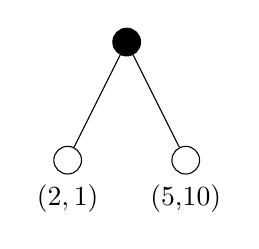
\begin{tikzpicture}
\tikzset{
solid node/.style={circle,draw,inner sep=1.5,minimum size=10pt,fill=black},
hollow node/.style={circle,draw,inner sep=1.5,minimum size=10pt}
}

\node(0)[solid node]{}
    child{node[hollow node,label=below:{$(2,1)$}]{}}
    child{node[hollow node,label=below:{(5,10)}]{}};
\end{tikzpicture}
\end{center}
\end{example}

In the following text
we restrict ourselves to two player games in which players alternate in
taking actions.

\subsection{Zero-sum games and minimax}

In zero-sum games one player wins at the cost of the other losing.
There are plenty of examples of such games, e.g., Chess, Go, which makes
them an important subject of study.

\begin{definition}
    Let $G = (N, S, s_0, F, A, E, \Delta, \rho, u)$ be a game.
    $G$ is said to be {\em zero-sum} if the rewards always sum to zero,
    that is $\sum_{i \in N} u_i(s) = 0$ for all $s \in F$.
\end{definition}

An important type of strategy is {\em minimax}. A player playing this
strategy is minimizing their potential maximum loss\footnote{Some might
prefer calling it {\em maximin} for maximization of the minimum reward,
which is equivalent to the first definition in zero-sum games.}. If both players play a
minimax strategy, the strategy profile is a Nash
equilibrium\footnote{
A strategic profile is a Nash equilibrium, if no player can get a higher
reward by switching a strategy.
    }$^,$\footnote{The {\em minimax theorem} was proven by John
von Neumann.}.

The {\em minimax algorithm} computes the value of each leaf in a game
tree assuming the opponent tries to harm the player as much as
possible. That is if player $1$ is computing which turn to play,
she uses the fact that she can maximize her profit in her future turns
but assumes player $2$ will try to minimize it.
After all options are computed in this alternating manner,
player $1$ plays the action going into the subtree with the highest value node.

Now we use the zero-sum property and our assumption of alternating turns
to simplify the algorithm for zero-sum games in two steps.

First, only a single payoff function can be used,
let it be $u_1$. Now higher values mean player 1 is winning and lower
values that player 2 is winning.
Thus player 1 maximizes in her turns, expects
player 2 to minimize in his turns.
Player 2 minimizes in his turns, expects
player 1 to maximize in her turns.

Second, instead of alternating between maximization and minimization, an
algorithm can always maximize if it alters the sign of the value in each
step.

These simplifications result in \autoref{negamax}, the {\em negamax
algorithm}.
Player 1 gets the value by evaluating
\textsc{Negamax}$($state$, 0)$,
player 2 gets the value by evaluating $-$\textsc{Negamax}$($state$, 1)$.

An example execution of the algorithm can be seen on a game of
tic-tac-toe in \autoref{fig:negamax}.
X is the first player, O is the second player. At the beginning X can
place her mark in the middle of the board and win, or place it at the
bottom and lose. The left branch has value 1, the right branch has value
$-1$.

% I read about the topic here:
% http://www.hamedahmadi.com/gametree/#negamax
% https://en.wikipedia.org/wiki/Minimax
% https://github.com/soratobukuroneko/tictactoe-negamax/blob/master/tictactoe.c
% https://neverstopbuilding-dropblog.herokuapp.com/minimax

\begin{algorithm}
\caption{Negamax}
\label{negamax}
\begin{algorithmic}
\Input Two-player zero-sum game\footnote{The $player$
numbers are shifted down by one for easy manipulation.}
$(N, S, s_0, F, A, E, \Delta, \rho, u)$, where players
 alternate in taking actions.
\Output Maximum payoff for player 0, its negation for player 1.
\Function{negamax}{$state, player$}
    \If{$state \in F$, i.e. a leaf in the game tree}
    \State \Return\footnote{The
    $[1,-1][player]$ evaluates to 1 for player 0 and to $-1$ for player 1.}
        $[1,-1][player] \cdot u_1(state)$
        otherwise
    \EndIf
    \State \Return $\max \{ - \Call{negamax}{child, 1 - player}
        \mid
        child \text{ of } state\footnote{Precisely
        for all enabled actions $a \in E(state)$ every $child \in \Delta(state, a)$.}
    \}$
\EndFunction
\end{algorithmic}
\end{algorithm}

\begin{figure}
% https://tex.stackexchange.com/questions/139782/creating-tic-tac-toe-boards-with-latex-tikz
\begin{forest}
  TTT/.style args={#1:#2}{
    make tab/.expanded=\forestove{content},
    label={\pgfkeysvalueof{/forest/label position #1}:$#2$}
  },
  TTT*/.style={
    make tab=::/::/::,
    content/.expand once=%
    \expandafter\vphantom\expandafter{\romannumeral-`0\forestov{content}},
    draw=none,
    append after command={(\tikzlastnode.north) edge (\tikzlastnode.south)},
    for descendants={before computing xy={l*=1.2}},
  },
  th/.style=thick,
  for tree={
    node options=draw,
    inner sep=+0pt,
    parent anchor=south,
    child anchor=north,
    l sep=0.7cm,
    s sep=1.7cm,
  },
  levellabel/.style={
    tikz+={
      \node [anchor=mid west] at (.mid -| levellabel coord) {#1};
    },
  },
  tikz+={
    \coordinate (levellabel coord) at (current bounding box.east);
  },
%
[o:o:x/x::o/x::o, TTT=r:{}, levellabel={\text{x's turn}, player = 0},
 [o:o:x/x:x:o/x::o, TTT=b:{\makecell[c]{(-1)\cdot 1 \\ \text{x wins}}},
   edge label={node[midway,left,font=\scriptsize]{$\cdot (-1)$}}]
   [o:o:x/x::o/x:x:o, TTT=r:{}, levellabel={\text{o's turn}, player = 1},
   edge label={node[midway,right,font=\scriptsize]{$\cdot (-1)$}},
   [o:o:x/x:o:o/x:x:o, TTT=b:{\makecell[c]{1\cdot (-1) \\ \text{o wins}}},
   levellabel={\phantom{\text{o's turn}, }player = 0},
   edge label={node[midway,right,font=\scriptsize]{$\cdot (-1)$}}]
 ]
]
\end{forest}
\caption{Negamax algorithm applied to tic-tac-toe.}
\label{fig:negamax}
\end{figure}

For larger games a variation called {\em minimax (negamax) search} is used, which
performs the computation only to a limited depth, and then uses
a heuristic to evaluate the last node it processes (unless it is a leaf).

\subsection{Solving with MCTS}

From the negamax algorithm in the previous section there is an easy step
to solving games with MCTS. \autoref{alg:mcts_negamax} is an
implementation of the Backup function in UCT for finding a good
action a player should take in a zero-sum game.

\begin{algorithm}
\caption{Negamax MCTS Backup}
\label{alg:mcts_negamax}
\begin{algorithmic}
\Function{backup}{$v, \Delta$}
    \While{$v$ is not $null$}
        \State $N(v) \gets N(v) + 1$
        \State $Q(v) \gets Q(v) + \Delta$
        \State $\Delta \gets - \Delta$
        \State $v \gets $ parent of $v$
    \EndWhile
\EndFunction
\end{algorithmic}
\end{algorithm}

% http://tim.hibal.org/blog/alpha-zero-how-and-why-it-works/

In comparison with minimax search MCTS may ignore unimportant
branches of the game tree and instead explore in greater detail the more
promising branches.

For example, when solving a tic-tac-toe game, the algorithm starts with
the current board state in the root of the tree, and then adds
the nodes representing the next possible states as its children.
They are explored with random rollouts, and the algorithm proceeds to
the parts of the tree which either seem to lead victory or which are
insufficiently explored. The balance between exploitation and
exploration is dependent on the choice of the constant in the tree
heuristic. See \parencite{mcts_ttt} for an elaborate explanation with
illustrations.

An important theoretical result is
that MCTS converges to minimax \parencite{Kocsis},
so eventually, after a lot of MCTS iterations, there is a negligible
difference between the results of the two methods and they pick the same
next move. However in
applications we want to know when to use minimax (\autoref{negamax}) and
when to use UCT (\autoref{alg:uct} with \autoref{alg:mcts_negamax}) without
iterating UCT for a long time.

While UCT achieved success in many games \parencite{mcts_survey},
for example in chess it does not perform well\footnote{
    Days prior to submitting this thesis a preprint article
    \parencite{alphazero} appeared,
describing a successful use of MCTS to play chess. The approach,
however, employs model-specific neural networks to guide the search and
so it seems that the observations made here (in tree traversal MCTS has
only a very limited information about the possible outcomes of each
choice) still translate to the domain of MDP
verification (as the models are usually not used again, it is not
effective to train a network for them). On the other hand this surely
deserves a deeper investigation.}. The reason being that chess
games contain a lot of trap states (states from which the opponent
has a guaranteed victory) which are reachable just in a few turns. UCT
then spends a lot of time exploring these unimportant parts of the search
tree \parencite{mcts_vs_chess}.

\subsection{Computer Go}

Go is an example of a game where MCTS has proven to be a good choice,
most recently with the AlphaGo program \parencite{alphago}.
We shortly introduce Go and compare it with chess where MCTS did not
achieve success.

The basic rules of Go are simple. The
standard board is a $9\times9$ (for beginners) or $19 \times 19$ grid.
Two players, black and white, alternate in their moves, each
placing a single stone of their color on an intersection of lines.
By surrounding the stones of the opponent a player captures all the
surrounded stones. The game ends when both players agree to end and the
winner is the player with the greater sum of controlled territory and
captured stones.
The rules are well explained in detail at
\href{http://playgo.to/iwtg/en/}{http://playgo.to/iwtg/en/}.

A Go player can observe that unlike in Chess there is seldom a quick way
to lose, as a loss of a small part of territory may be reversed, however
losing an important piece is hardly reversible.
This gives us an important example of games where MCTS performs well (in
Go it is worth exploring a plethora of moves) and where it does not
(e.g., in Chess, due to the trap states described above).
It seems plausible this
generalizes well to territory versus piece based games.

We end our detour to games with Arimaa, a game specifically designed in
2002 to be easy for humans but hard for computers, for example by
allowing more moves per turn. Eventually Arimaa players lost to a
program in 2015 \parencite{arimaa}. The program uses techniques similar
to chess programs like alpha-beta pruning and on top of that employs
heuristics inspired by the best human players. See \parencite{jakl} for
MCTS related insights into Arimaa.
